\documentclass[11pt]{beamer}
\title{Computing Linear Arithmetic Representation of Reachability Relation  of One-counter Automata}
\usepackage{verbatim}
\usepackage{amsmath}
\usepackage{amsthm}
\usepackage{listings}
\usepackage{graphics}
\usepackage{color}
\usepackage{stmaryrd}
\usepackage{multicol}
\usepackage{tabularx}
\usepackage{listings}
\usepackage{tikz}

\usetikzlibrary{automata,shapes,arrows,patterns,calc,positioning}
\tikzset{every picture/.style={->, >=stealth', shorten >=0pt, auto, initial text={}}}
\tikzstyle{flowchartelement} = [draw, inner sep=3pt, align=center]
\tikzstyle{inputoutput} = [flowchartelement, trapezium, trapezium right angle=-70pt, trapezium left angle=70pt]
\tikzstyle{test} = [flowchartelement, diamond]
\tikzstyle{code} = [flowchartelement, minimum width=20mm, rectangle]
\tikzstyle{connector} = [draw, circle, fill=black, inner sep=1.25pt]
\newtheorem{proposition}{Proposition}
\author{
    Authors: \textbf{Xie Li}, Taolue Chen, Zhilin Wu and Mingji Xia
}
\date{SETTA 2020: Guangzhou, China, November 24-28, 2020}

\begin{document}
\maketitle
\begin{frame}\frametitle{Overview}
\begin{itemize}
\item Introduction to One-counter Automata(OCA) and its Reachability Problem.
\pause
\item Computing the Reachability Relation of OCA.

\item Introduction to Tool \textsc{ORAReach}.

\item Experimental Results of our Tool \textsc{OCAReach}.

\end{itemize}
\end{frame}


\begin{frame}\frametitle{What is One-counter Automata(OCA)}
\begin{itemize}

\item DFA with a \textbf{counter} where counter value is \textbf{non-negative}.

\item Transitions: $q\stackrel{\texttt{Op}}{\rightarrow} q'$ where $\texttt{Op}\in \{\texttt{add}(+1), \texttt{add}(-1), \texttt{zero}\}$
\end{itemize}
\begin{example}[OCA]
\begin{center}
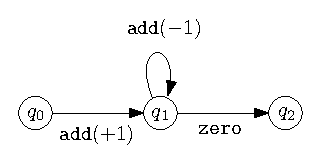
\includegraphics[scale=1]{ocaexample.eps}
\end{center}


\end{example}
Semantic of OCA: A transition system where the configuration is of the form $(q,c)$ and counter changes corresponds to OCA.

\[(q_1, c_1) \rightarrow_\mathcal{A} (q_2,c_2)\]

if $q_1 \stackrel{\texttt{add}(+1)}{\longrightarrow} q_2$ in the OCA and $c_1 + 1 = c2$, or

if $q_1 \stackrel{\texttt{zero}}{\longrightarrow} q_2$ and $c_1 = c_2 = 0$.
\end{frame}

\begin{frame}\frametitle{Reachability Problem of OCA}

\textbf{Reachability Problem of OCA: } whether $(q_s, c_s)\rightarrow^*_{\mathcal{A}} (q_t, c_t)$

\begin{example}\frametitle{Reachability}
\begin{multicols}{2}
\begin{center}
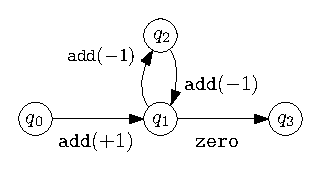
\includegraphics[scale=1]{reachexample.eps}
\end{center}
\begin{itemize}
\item  $(q_3, 0)$ is reachable from $(q_0, 1)$.
\item  $(q_3, 0)$ is not reachable from $(q_0, 0)$ 
\end{itemize}

\begin{center}
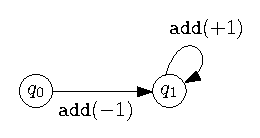
\includegraphics[scale=1]{reachexample2.eps}

\end{center}
Due to the non-negative requirement,

$(q_1, 1)$ is not reachable from $(q_0, 0)$



\end{multicols}

\end{example}
\end{frame}


\begin{frame}\frametitle{Weighted Directed Graph,  Path Flow and Support}
\begin{itemize}

\item An OCA can be regarded as a weighted directed graph $G_\mathcal{A} = (V,E,\eta)$.

\item \textbf{Path}: a sequence of vertices $v_0\cdot v_1 \cdots v_k$ where $(v_i, v_{i+1}) \in E$.
\begin{itemize}
\item Weight of path
\item Drop of path
\end{itemize}
\item \textbf{Flow}: a function $f: E\rightarrow \mathbb{N}$.
\end{itemize}

\begin{example}
\begin{center}
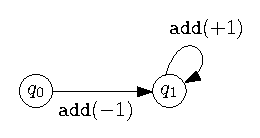
\includegraphics[scale=1]{reachexample2.eps}
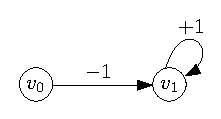
\includegraphics[scale=1]{wg.eps}
\begin{itemize}

\item path: $v_0\cdot v_1\cdot v_1$
\item weight: $+1$
\item drop: $-1$
\end{itemize}
\end{center}


\end{example}
\end{frame}

\begin{frame}\frametitle{Path Flow and Support}


\begin{itemize}

\item  $s$-$t$ \textbf{path flow}: the flow corresponds to a path.

\item Support: edge-induced subgraph of path.
\end{itemize}


\begin{example}
\begin{multicols}{2}

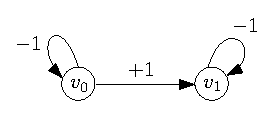
\includegraphics[scale=1]{wg2.eps}
\begin{itemize}

\item Support: 

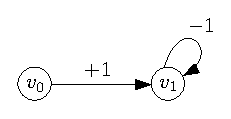
\includegraphics[scale=1]{support.eps}

\item Path: $v_0\cdot v_1\cdot v_1$

\item Pathflow: $f(v_0,v_0) = 0$ 

$f(v_0,v_1) = 1$

$ f(v_1,v_1) = 2$

\item Weight: $w = \Sigma_{e\in E} f(e)\cdot \eta(e)$
\end{itemize}
\end{multicols}

\end{example}


\end{frame}


\begin{frame}\frametitle{The Difficulty of the Reachability Problem}
\begin{center}
\large
\textbf{NON-NEGATIVE}
\end{center}
If we do not require the non-negative of counter.

\begin{itemize}
\item Flow is a path flow $\Leftrightarrow$ Requirements on flow.
\begin{itemize}
\item $v_s\cdots v_t$ where $s \ne t$

\item $v_s\cdots v_s$
\end{itemize}
\item Weight equals to the value change.
\end{itemize}

\textbf{Non-negative} implies the constraint:
everywhere along the path, the counter need to be non-negative.
\end{frame}

\begin{frame}\frametitle{Certificate of the Reachability}

Use \textbf{path flow} as certificate of OCA reachability problem.

\begin{itemize}
\item Type 1 Certificate: 

\item Type 2 Certificate

\item Type 3 Certificate
\end{itemize}


\end{frame}


\begin{frame}\frametitle{Edge Decomposition}

\end{frame}


\begin{frame}\frametitle{Reachability Relation of OCA}

\textbf{Reachability Relation of OCA}: 
\[\phi_{{\mathcal{A}}, q_s, q_t}(x_s, x_t)\]

\end{frame}


	

\begin{frame}\frametitle{How we Reduce the Reachability Relation to QFPA Formula}

\end{frame}

\begin{frame}\frametitle{\textsc{OCAReach}: Architecture}

\end{frame}

\begin{frame}\frametitle{Experimental Evaluation}

\end{frame}

\end{document}